\documentclass[1p]{elsarticle_modified}
%\bibliographystyle{elsarticle-num}

%\usepackage[colorlinks]{hyperref}
%\usepackage{abbrmath_seonhwa} %\Abb, \Ascr, \Acal ,\Abf, \Afrak
\usepackage{amsfonts}
\usepackage{amssymb}
\usepackage{amsmath}
\usepackage{amsthm}
\usepackage{scalefnt}
\usepackage{amsbsy}
\usepackage{kotex}
\usepackage{caption}
\usepackage{subfig}
\usepackage{color}
\usepackage{graphicx}
\usepackage{xcolor} %% white, black, red, green, blue, cyan, magenta, yellow
\usepackage{float}
\usepackage{setspace}
\usepackage{hyperref}

\usepackage{tikz}
\usetikzlibrary{arrows}

\usepackage{multirow}
\usepackage{array} % fixed length table
\usepackage{hhline}

%%%%%%%%%%%%%%%%%%%%%
\makeatletter
\renewcommand*\env@matrix[1][\arraystretch]{%
	\edef\arraystretch{#1}%
	\hskip -\arraycolsep
	\let\@ifnextchar\new@ifnextchar
	\array{*\c@MaxMatrixCols c}}
\makeatother %https://tex.stackexchange.com/questions/14071/how-can-i-increase-the-line-spacing-in-a-matrix
%%%%%%%%%%%%%%%

\usepackage[normalem]{ulem}

\newcommand{\msout}[1]{\ifmmode\text{\sout{\ensuremath{#1}}}\else\sout{#1}\fi}
%SOURCE: \msout is \stkout macro in https://tex.stackexchange.com/questions/20609/strikeout-in-math-mode

\newcommand{\cancel}[1]{
	\ifmmode
	{\color{red}\msout{#1}}
	\else
	{\color{red}\sout{#1}}
	\fi
}

\newcommand{\add}[1]{
	{\color{blue}\uwave{#1}}
}

\newcommand{\replace}[2]{
	\ifmmode
	{\color{red}\msout{#1}}{\color{blue}\uwave{#2}}
	\else
	{\color{red}\sout{#1}}{\color{blue}\uwave{#2}}
	\fi
}

\newcommand{\Sol}{\mathcal{S}} %segment
\newcommand{\D}{D} %diagram
\newcommand{\A}{\mathcal{A}} %arc


%%%%%%%%%%%%%%%%%%%%%%%%%%%%%5 test

\def\sl{\operatorname{\textup{SL}}(2,\Cbb)}
\def\psl{\operatorname{\textup{PSL}}(2,\Cbb)}
\def\quan{\mkern 1mu \triangleright \mkern 1mu}

\theoremstyle{definition}
\newtheorem{thm}{Theorem}[section]
\newtheorem{prop}[thm]{Proposition}
\newtheorem{lem}[thm]{Lemma}
\newtheorem{ques}[thm]{Question}
\newtheorem{cor}[thm]{Corollary}
\newtheorem{defn}[thm]{Definition}
\newtheorem{exam}[thm]{Example}
\newtheorem{rmk}[thm]{Remark}
\newtheorem{alg}[thm]{Algorithm}

\newcommand{\I}{\sqrt{-1}}
\begin{document}

%\begin{frontmatter}
%
%\title{Boundary parabolic representations of knots up to 8 crossings}
%
%%% Group authors per affiliation:
%\author{Yunhi Cho} 
%\address{Department of Mathematics, University of Seoul, Seoul, Korea}
%\ead{yhcho@uos.ac.kr}
%
%
%\author{Seonhwa Kim} %\fnref{s_kim}}
%\address{Center for Geometry and Physics, Institute for Basic Science, Pohang, 37673, Korea}
%\ead{ryeona17@ibs.re.kr}
%
%\author{Hyuk Kim}
%\address{Department of Mathematical Sciences, Seoul National University, Seoul 08826, Korea}
%\ead{hyukkim@snu.ac.kr}
%
%\author{Seokbeom Yoon}
%\address{Department of Mathematical Sciences, Seoul National University, Seoul, 08826,  Korea}
%\ead{sbyoon15@snu.ac.kr}
%
%\begin{abstract}
%We find all boundary parabolic representation of knots up to 8 crossings.
%
%\end{abstract}
%\begin{keyword}
%    \MSC[2010] 57M25 
%\end{keyword}
%
%\end{frontmatter}

%\linenumbers
%\tableofcontents
%
\newcommand\colored[1]{\textcolor{white}{\rule[-0.35ex]{0.8em}{1.4ex}}\kern-0.8em\color{red} #1}%
%\newcommand\colored[1]{\textcolor{white}{ #1}\kern-2.17ex	\textcolor{white}{ #1}\kern-1.81ex	\textcolor{white}{ #1}\kern-2.15ex\color{red}#1	}

{\Large $\underline{12a_{0851}~(K12a_{0851})}$}

\setlength{\tabcolsep}{10pt}
\renewcommand{\arraystretch}{1.6}
\vspace{1cm}\begin{tabular}{m{100pt}>{\centering\arraybackslash}m{274pt}}
\multirow{5}{120pt}{
	\centering
	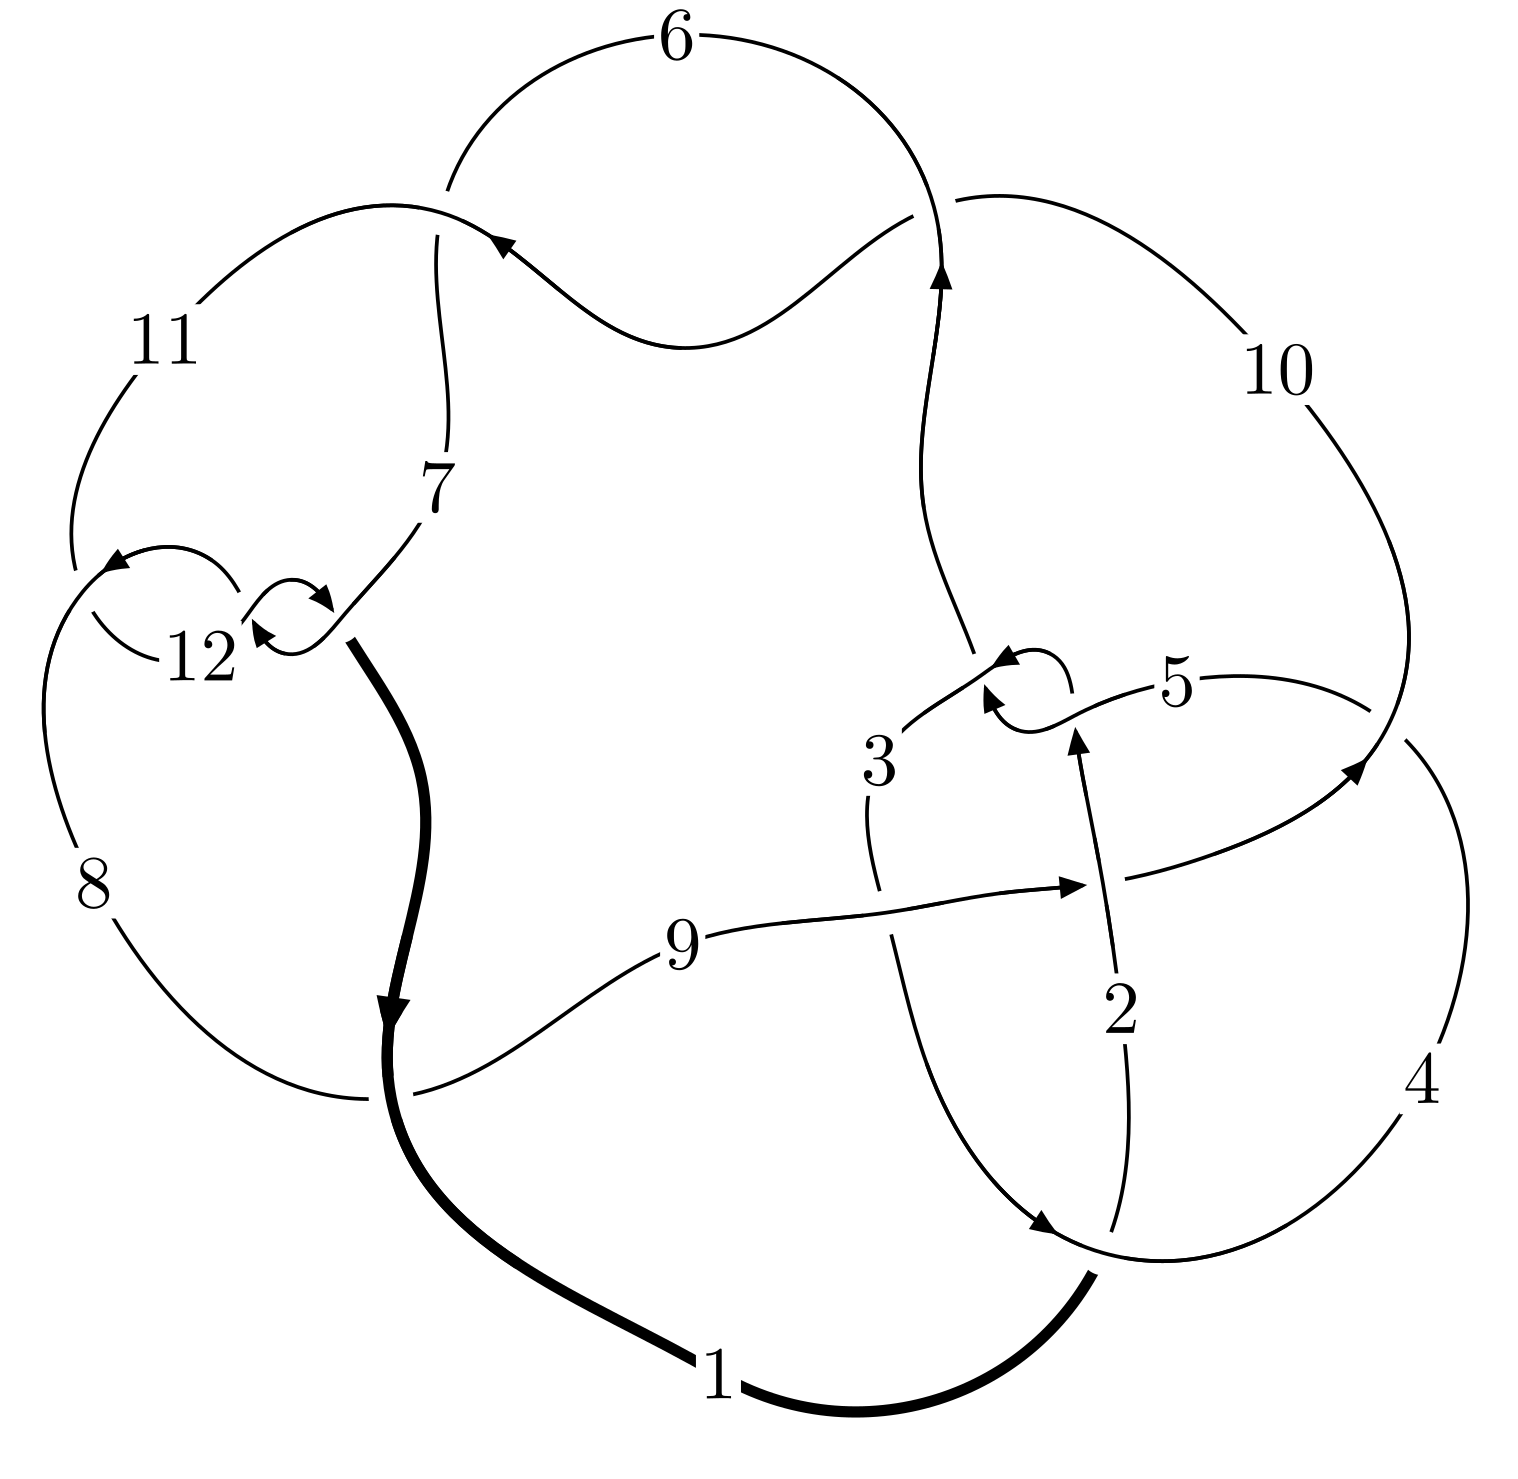
\includegraphics[width=112pt]{../../../GIT/diagram.site/Diagrams/png/1652_12a_0851.png}\\
\ \ \ A knot diagram\footnotemark}&
\allowdisplaybreaks
\textbf{Linearized knot diagam} \\
\cline{2-2}
 &
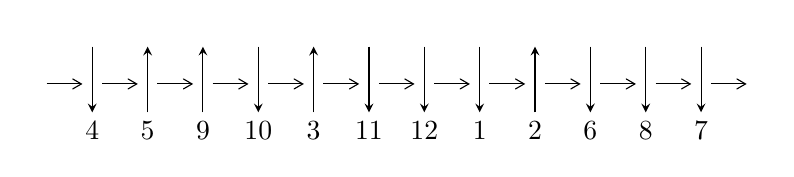
\begin{tikzpicture}[x=20pt, y=17pt]
	% nodes
	\node (C0) at (0, 0) {};
	\node (C1) at (1, 0) {};
	\node (C1U) at (1, +1) {};
	\node (C1D) at (1, -1) {4};

	\node (C2) at (2, 0) {};
	\node (C2U) at (2, +1) {};
	\node (C2D) at (2, -1) {5};

	\node (C3) at (3, 0) {};
	\node (C3U) at (3, +1) {};
	\node (C3D) at (3, -1) {9};

	\node (C4) at (4, 0) {};
	\node (C4U) at (4, +1) {};
	\node (C4D) at (4, -1) {10};

	\node (C5) at (5, 0) {};
	\node (C5U) at (5, +1) {};
	\node (C5D) at (5, -1) {3};

	\node (C6) at (6, 0) {};
	\node (C6U) at (6, +1) {};
	\node (C6D) at (6, -1) {11};

	\node (C7) at (7, 0) {};
	\node (C7U) at (7, +1) {};
	\node (C7D) at (7, -1) {12};

	\node (C8) at (8, 0) {};
	\node (C8U) at (8, +1) {};
	\node (C8D) at (8, -1) {1};

	\node (C9) at (9, 0) {};
	\node (C9U) at (9, +1) {};
	\node (C9D) at (9, -1) {2};

	\node (C10) at (10, 0) {};
	\node (C10U) at (10, +1) {};
	\node (C10D) at (10, -1) {6};

	\node (C11) at (11, 0) {};
	\node (C11U) at (11, +1) {};
	\node (C11D) at (11, -1) {8};

	\node (C12) at (12, 0) {};
	\node (C12U) at (12, +1) {};
	\node (C12D) at (12, -1) {7};
	\node (C13) at (13, 0) {};

	% arrows
	\draw[->,>={angle 60}]
	(C0) edge (C1) (C1) edge (C2) (C2) edge (C3) (C3) edge (C4) (C4) edge (C5) (C5) edge (C6) (C6) edge (C7) (C7) edge (C8) (C8) edge (C9) (C9) edge (C10) (C10) edge (C11) (C11) edge (C12) (C12) edge (C13) ;	\draw[->,>=stealth]
	(C1U) edge (C1D) (C2D) edge (C2U) (C3D) edge (C3U) (C4U) edge (C4D) (C5D) edge (C5U) (C6U) edge (C6D) (C7U) edge (C7D) (C8U) edge (C8D) (C9D) edge (C9U) (C10U) edge (C10D) (C11U) edge (C11D) (C12U) edge (C12D) ;
	\end{tikzpicture} \\
\hhline{~~} \\& 
\textbf{Solving Sequence} \\ \cline{2-2} 
 &
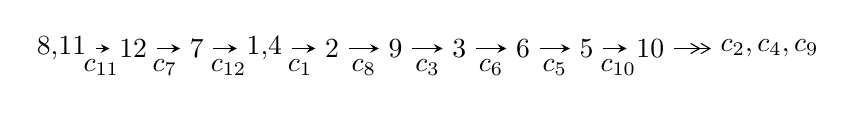
\begin{tikzpicture}[x=23pt, y=7pt]
	% node
	\node (A0) at (-1/8, 0) {8,11};
	\node (A1) at (1, 0) {12};
	\node (A2) at (2, 0) {7};
	\node (A3) at (49/16, 0) {1,4};
	\node (A4) at (33/8, 0) {2};
	\node (A5) at (41/8, 0) {9};
	\node (A6) at (49/8, 0) {3};
	\node (A7) at (57/8, 0) {6};
	\node (A8) at (65/8, 0) {5};
	\node (A9) at (73/8, 0) {10};
	\node (C1) at (1/2, -1) {$c_{11}$};
	\node (C2) at (3/2, -1) {$c_{7}$};
	\node (C3) at (5/2, -1) {$c_{12}$};
	\node (C4) at (29/8, -1) {$c_{1}$};
	\node (C5) at (37/8, -1) {$c_{8}$};
	\node (C6) at (45/8, -1) {$c_{3}$};
	\node (C7) at (53/8, -1) {$c_{6}$};
	\node (C8) at (61/8, -1) {$c_{5}$};
	\node (C9) at (69/8, -1) {$c_{10}$};
	\node (A10) at (11, 0) {$c_{2},c_{4},c_{9}$};

	% edge
	\draw[->,>=stealth]	
	(A0) edge (A1) (A1) edge (A2) (A2) edge (A3) (A3) edge (A4) (A4) edge (A5) (A5) edge (A6) (A6) edge (A7) (A7) edge (A8) (A8) edge (A9) ;
	\draw[->>,>={angle 60}]	
	(A9) edge (A10);
\end{tikzpicture} \\ 

\end{tabular} \\

\footnotetext{
The image of knot diagram is generated by the software ``\textbf{Draw programme}" developed by Andrew Bartholomew(\url{http://www.layer8.co.uk/maths/draw/index.htm\#Running-draw}), where we modified some parts for our purpose(\url{https://github.com/CATsTAILs/LinksPainter}).
}\phantom \\ \newline 
\centering \textbf{Ideals for irreducible components\footnotemark of $X_{\text{par}}$} 
 
\begin{align*}
I^u_{1}&=\langle 
1.96995\times10^{27} u^{83}+4.01738\times10^{27} u^{82}+\cdots+7.57665\times10^{26} b+2.90943\times10^{27},\\
\phantom{I^u_{1}}&\phantom{= \langle  }3.36403\times10^{27} u^{83}+4.75814\times10^{27} u^{82}+\cdots+7.57665\times10^{26} a+8.28011\times10^{27},\;u^{84}+2 u^{83}+\cdots+u+1\rangle \\
I^u_{2}&=\langle 
u^2+b+1,\;u^2+a+2,\;u^3+u^2+2 u+1\rangle \\
\\
\end{align*}
\raggedright * 2 irreducible components of $\dim_{\mathbb{C}}=0$, with total 87 representations.\\
\footnotetext{All coefficients of polynomials are rational numbers. But the coefficients are sometimes approximated in decimal forms when there is not enough margin.}
\newpage
\renewcommand{\arraystretch}{1}
\centering \section*{I. $I^u_{1}= \langle 1.97\times10^{27} u^{83}+4.02\times10^{27} u^{82}+\cdots+7.58\times10^{26} b+2.91\times10^{27},\;3.36\times10^{27} u^{83}+4.76\times10^{27} u^{82}+\cdots+7.58\times10^{26} a+8.28\times10^{27},\;u^{84}+2 u^{83}+\cdots+u+1 \rangle$}
\flushleft \textbf{(i) Arc colorings}\\
\begin{tabular}{m{7pt} m{180pt} m{7pt} m{180pt} }
\flushright $a_{8}=$&$\begin{pmatrix}0\\u\end{pmatrix}$ \\
\flushright $a_{11}=$&$\begin{pmatrix}1\\0\end{pmatrix}$ \\
\flushright $a_{12}=$&$\begin{pmatrix}1\\u^2\end{pmatrix}$ \\
\flushright $a_{7}=$&$\begin{pmatrix}u\\u^3+u\end{pmatrix}$ \\
\flushright $a_{1}=$&$\begin{pmatrix}u^2+1\\u^4+2 u^2\end{pmatrix}$ \\
\flushright $a_{4}=$&$\begin{pmatrix}-4.44000 u^{83}-6.28001 u^{82}+\cdots+13.8326 u-10.9285\\-2.60003 u^{83}-5.30231 u^{82}+\cdots+4.48846 u-3.84000\end{pmatrix}$ \\
\flushright $a_{2}=$&$\begin{pmatrix}1.40000 u^{83}+2.40001 u^{82}+\cdots-3.79679 u+2.51127\\0.399993 u^{83}-0.0251959 u^{82}+\cdots-1.11127 u+1.40000\end{pmatrix}$ \\
\flushright $a_{9}=$&$\begin{pmatrix}- u^5-2 u^3- u\\- u^7-3 u^5-2 u^3+u\end{pmatrix}$ \\
\flushright $a_{3}=$&$\begin{pmatrix}-3.44000 u^{83}-4.07994 u^{82}+\cdots+11.1855 u-8.67404\\-2.60000 u^{83}-5.37729 u^{82}+\cdots+6.07404 u-5.44000\end{pmatrix}$ \\
\flushright $a_{6}=$&$\begin{pmatrix}u^3+2 u\\u^3+u\end{pmatrix}$ \\
\flushright $a_{5}=$&$\begin{pmatrix}-2.84000 u^{83}-3.08004 u^{82}+\cdots+10.4753 u-7.72107\\-2.40000 u^{83}-5.07341 u^{82}+\cdots+6.32107 u-4.84000\end{pmatrix}$ \\
\flushright $a_{10}=$&$\begin{pmatrix}- u^6-3 u^4-2 u^2+1\\- u^6-2 u^4- u^2\end{pmatrix}$\\&\end{tabular}
\flushleft \textbf{(ii) Obstruction class $= -1$}\\~\\
\flushleft \textbf{(iii) Cusp Shapes $= -\frac{166187238455782666427778654}{757665015935352679203803969} u^{83}-\frac{2271996256671495868603397318}{757665015935352679203803969} u^{82}+\cdots-\frac{32408113859025183515073838511}{757665015935352679203803969} u+\frac{15078033543060885625800068293}{757665015935352679203803969}$}\\~\\
\newpage\renewcommand{\arraystretch}{1}
\flushleft \textbf{(iv) u-Polynomials at the component}\newline \\
\begin{tabular}{m{50pt}|m{274pt}}
Crossings & \hspace{64pt}u-Polynomials at each crossing \\
\hline $$\begin{aligned}c_{1}\end{aligned}$$&$\begin{aligned}
&u^{84}-13 u^{83}+\cdots-36 u+8
\end{aligned}$\\
\hline $$\begin{aligned}c_{2},c_{5}\end{aligned}$$&$\begin{aligned}
&u^{84}+4 u^{83}+\cdots-24 u-1
\end{aligned}$\\
\hline $$\begin{aligned}c_{3}\end{aligned}$$&$\begin{aligned}
&u^{84}- u^{83}+\cdots+3950 u+817
\end{aligned}$\\
\hline $$\begin{aligned}c_{4}\end{aligned}$$&$\begin{aligned}
&u^{84}+u^{83}+\cdots+6 u-1
\end{aligned}$\\
\hline $$\begin{aligned}c_{6},c_{8},c_{10}\end{aligned}$$&$\begin{aligned}
&u^{84}-2 u^{83}+\cdots+69 u+17
\end{aligned}$\\
\hline $$\begin{aligned}c_{7},c_{11},c_{12}\end{aligned}$$&$\begin{aligned}
&u^{84}+2 u^{83}+\cdots+u+1
\end{aligned}$\\
\hline $$\begin{aligned}c_{9}\end{aligned}$$&$\begin{aligned}
&u^{84}+2 u^{83}+\cdots- u-1
\end{aligned}$\\
\hline
\end{tabular}\\~\\
\newpage\renewcommand{\arraystretch}{1}
\flushleft \textbf{(v) Riley Polynomials at the component}\newline \\
\begin{tabular}{m{50pt}|m{274pt}}
Crossings & \hspace{64pt}Riley Polynomials at each crossing \\
\hline $$\begin{aligned}c_{1}\end{aligned}$$&$\begin{aligned}
&y^{84}-21 y^{83}+\cdots-1232 y+64
\end{aligned}$\\
\hline $$\begin{aligned}c_{2},c_{5}\end{aligned}$$&$\begin{aligned}
&y^{84}-48 y^{83}+\cdots-224 y+1
\end{aligned}$\\
\hline $$\begin{aligned}c_{3}\end{aligned}$$&$\begin{aligned}
&y^{84}+85 y^{83}+\cdots+14128130 y+667489
\end{aligned}$\\
\hline $$\begin{aligned}c_{4}\end{aligned}$$&$\begin{aligned}
&y^{84}+69 y^{83}+\cdots-234 y+1
\end{aligned}$\\
\hline $$\begin{aligned}c_{6},c_{8},c_{10}\end{aligned}$$&$\begin{aligned}
&y^{84}-86 y^{83}+\cdots-8807 y+289
\end{aligned}$\\
\hline $$\begin{aligned}c_{7},c_{11},c_{12}\end{aligned}$$&$\begin{aligned}
&y^{84}+66 y^{83}+\cdots-7 y+1
\end{aligned}$\\
\hline $$\begin{aligned}c_{9}\end{aligned}$$&$\begin{aligned}
&y^{84}-14 y^{83}+\cdots-7 y+1
\end{aligned}$\\
\hline
\end{tabular}\\~\\
\newpage\flushleft \textbf{(vi) Complex Volumes and Cusp Shapes}
$$\begin{array}{c|c|c}  
\text{Solutions to }I^u_{1}& \I (\text{vol} + \sqrt{-1}CS) & \text{Cusp shape}\\
 \hline 
\begin{aligned}
u &= \phantom{-}0.110255 + 0.992663 I \\
a &= -0.879103 + 0.499853 I \\
b &= -0.471696 + 0.417164 I\end{aligned}
 & -0.328989 + 0.984245 I & \phantom{-0.000000 } 0 \\ \hline\begin{aligned}
u &= \phantom{-}0.110255 - 0.992663 I \\
a &= -0.879103 - 0.499853 I \\
b &= -0.471696 - 0.417164 I\end{aligned}
 & -0.328989 - 0.984245 I & \phantom{-0.000000 } 0 \\ \hline\begin{aligned}
u &= -0.299517 + 0.904327 I \\
a &= \phantom{-}0.653627 - 0.164395 I \\
b &= \phantom{-}0.784926 - 0.330738 I\end{aligned}
 & \phantom{-}1.86898 + 5.21583 I & \phantom{-0.000000 } 0 \\ \hline\begin{aligned}
u &= -0.299517 - 0.904327 I \\
a &= \phantom{-}0.653627 + 0.164395 I \\
b &= \phantom{-}0.784926 + 0.330738 I\end{aligned}
 & \phantom{-}1.86898 - 5.21583 I & \phantom{-0.000000 } 0 \\ \hline\begin{aligned}
u &= \phantom{-}0.897832 + 0.024492 I \\
a &= -2.22947 + 0.33832 I \\
b &= -2.32818 + 0.38487 I\end{aligned}
 & -9.21782 - 0.46343 I & -10.71619 - 2.01137 I \\ \hline\begin{aligned}
u &= \phantom{-}0.897832 - 0.024492 I \\
a &= -2.22947 - 0.33832 I \\
b &= -2.32818 - 0.38487 I\end{aligned}
 & -9.21782 + 0.46343 I & -10.71619 + 2.01137 I \\ \hline\begin{aligned}
u &= -0.891180 + 0.064032 I \\
a &= -3.33093 + 0.18661 I \\
b &= -3.33496 + 0.25333 I\end{aligned}
 & -6.55361 + 12.23930 I & -7.27322 - 7.00359 I \\ \hline\begin{aligned}
u &= -0.891180 - 0.064032 I \\
a &= -3.33093 - 0.18661 I \\
b &= -3.33496 - 0.25333 I\end{aligned}
 & -6.55361 - 12.23930 I & -7.27322 + 7.00359 I \\ \hline\begin{aligned}
u &= -0.883835 + 0.038054 I \\
a &= \phantom{-}3.58891 - 0.56439 I \\
b &= \phantom{-}3.46927 - 0.50941 I\end{aligned}
 & -9.90913 + 5.72369 I & -9.95611 - 4.95013 I \\ \hline\begin{aligned}
u &= -0.883835 - 0.038054 I \\
a &= \phantom{-}3.58891 + 0.56439 I \\
b &= \phantom{-}3.46927 + 0.50941 I\end{aligned}
 & -9.90913 - 5.72369 I & -9.95611 + 4.95013 I\\
 \hline 
 \end{array}$$\newpage$$\begin{array}{c|c|c}  
\text{Solutions to }I^u_{1}& \I (\text{vol} + \sqrt{-1}CS) & \text{Cusp shape}\\
 \hline 
\begin{aligned}
u &= \phantom{-}0.878158 + 0.070546 I \\
a &= \phantom{-}1.87000 - 0.49822 I \\
b &= \phantom{-}1.77275 - 0.49012 I\end{aligned}
 & -7.77096 - 4.58033 I & -9.29631 + 5.11031 I \\ \hline\begin{aligned}
u &= \phantom{-}0.878158 - 0.070546 I \\
a &= \phantom{-}1.87000 + 0.49822 I \\
b &= \phantom{-}1.77275 + 0.49012 I\end{aligned}
 & -7.77096 + 4.58033 I & -9.29631 - 5.11031 I \\ \hline\begin{aligned}
u &= \phantom{-}0.866332 + 0.010497 I \\
a &= \phantom{-}1.40515 + 2.06321 I \\
b &= \phantom{-}1.41089 + 2.80011 I\end{aligned}
 & -5.88867 - 0.76646 I & -10.18802 - 8.51416 I \\ \hline\begin{aligned}
u &= \phantom{-}0.866332 - 0.010497 I \\
a &= \phantom{-}1.40515 - 2.06321 I \\
b &= \phantom{-}1.41089 - 2.80011 I\end{aligned}
 & -5.88867 + 0.76646 I & -10.18802 + 8.51416 I \\ \hline\begin{aligned}
u &= -0.858093 + 0.025331 I \\
a &= -0.95600 - 2.32630 I \\
b &= -0.93847 - 1.67793 I\end{aligned}
 & -4.28941 + 3.74724 I & -4.52184 - 5.72401 I \\ \hline\begin{aligned}
u &= -0.858093 - 0.025331 I \\
a &= -0.95600 + 2.32630 I \\
b &= -0.93847 + 1.67793 I\end{aligned}
 & -4.28941 - 3.74724 I & -4.52184 + 5.72401 I \\ \hline\begin{aligned}
u &= -0.845503\phantom{ +0.000000I} \\
a &= -4.49525\phantom{ +0.000000I} \\
b &= -4.08680\phantom{ +0.000000I}\end{aligned}
 & -2.58884\phantom{ +0.000000I} & -1.97210\phantom{ +0.000000I} \\ \hline\begin{aligned}
u &= -0.087999 + 1.205740 I \\
a &= \phantom{-}0.851450 + 0.079273 I \\
b &= \phantom{-}0.72162 - 1.91902 I\end{aligned}
 & \phantom{-}3.95448 + 1.52948 I & \phantom{-0.000000 } 0 \\ \hline\begin{aligned}
u &= -0.087999 - 1.205740 I \\
a &= \phantom{-}0.851450 - 0.079273 I \\
b &= \phantom{-}0.72162 + 1.91902 I\end{aligned}
 & \phantom{-}3.95448 - 1.52948 I & \phantom{-0.000000 } 0 \\ \hline\begin{aligned}
u &= \phantom{-}0.317565 + 0.699615 I \\
a &= \phantom{-}0.591065 - 0.420702 I \\
b &= \phantom{-}0.719031 - 0.569754 I\end{aligned}
 & \phantom{-}2.21608 + 5.47917 I & -2.75820 - 3.97142 I\\
 \hline 
 \end{array}$$\newpage$$\begin{array}{c|c|c}  
\text{Solutions to }I^u_{1}& \I (\text{vol} + \sqrt{-1}CS) & \text{Cusp shape}\\
 \hline 
\begin{aligned}
u &= \phantom{-}0.317565 - 0.699615 I \\
a &= \phantom{-}0.591065 + 0.420702 I \\
b &= \phantom{-}0.719031 + 0.569754 I\end{aligned}
 & \phantom{-}2.21608 - 5.47917 I & -2.75820 + 3.97142 I \\ \hline\begin{aligned}
u &= \phantom{-}0.021059 + 1.251870 I \\
a &= \phantom{-}0.240736 + 0.329853 I \\
b &= \phantom{-}0.90373 - 1.23188 I\end{aligned}
 & \phantom{-}4.24491 + 1.49996 I & \phantom{-0.000000 } 0 \\ \hline\begin{aligned}
u &= \phantom{-}0.021059 - 1.251870 I \\
a &= \phantom{-}0.240736 - 0.329853 I \\
b &= \phantom{-}0.90373 + 1.23188 I\end{aligned}
 & \phantom{-}4.24491 - 1.49996 I & \phantom{-0.000000 } 0 \\ \hline\begin{aligned}
u &= -0.181517 + 1.243580 I \\
a &= \phantom{-}0.515986 + 0.448015 I \\
b &= \phantom{-}0.940034 + 0.122735 I\end{aligned}
 & \phantom{-}2.79988 + 2.45137 I & \phantom{-0.000000 } 0 \\ \hline\begin{aligned}
u &= -0.181517 - 1.243580 I \\
a &= \phantom{-}0.515986 - 0.448015 I \\
b &= \phantom{-}0.940034 - 0.122735 I\end{aligned}
 & \phantom{-}2.79988 - 2.45137 I & \phantom{-0.000000 } 0 \\ \hline\begin{aligned}
u &= -0.138549 + 1.255270 I \\
a &= -2.68245 + 0.16980 I \\
b &= -1.20511 + 3.23411 I\end{aligned}
 & \phantom{-}4.81134 + 2.18966 I & \phantom{-0.000000 } 0 \\ \hline\begin{aligned}
u &= -0.138549 - 1.255270 I \\
a &= -2.68245 - 0.16980 I \\
b &= -1.20511 - 3.23411 I\end{aligned}
 & \phantom{-}4.81134 - 2.18966 I & \phantom{-0.000000 } 0 \\ \hline\begin{aligned}
u &= -0.695609 + 0.224245 I \\
a &= -0.419849 - 0.863366 I \\
b &= -0.303627 - 0.104607 I\end{aligned}
 & -0.17080 - 1.42571 I & -7.44428 + 4.45956 I \\ \hline\begin{aligned}
u &= -0.695609 - 0.224245 I \\
a &= -0.419849 + 0.863366 I \\
b &= -0.303627 + 0.104607 I\end{aligned}
 & -0.17080 + 1.42571 I & -7.44428 - 4.45956 I \\ \hline\begin{aligned}
u &= \phantom{-}0.427785 + 1.209710 I \\
a &= -0.848570 + 0.981327 I \\
b &= -1.31346 - 0.86465 I\end{aligned}
 & -4.26362 - 0.09192 I & \phantom{-0.000000 } 0\\
 \hline 
 \end{array}$$\newpage$$\begin{array}{c|c|c}  
\text{Solutions to }I^u_{1}& \I (\text{vol} + \sqrt{-1}CS) & \text{Cusp shape}\\
 \hline 
\begin{aligned}
u &= \phantom{-}0.427785 - 1.209710 I \\
a &= -0.848570 - 0.981327 I \\
b &= -1.31346 + 0.86465 I\end{aligned}
 & -4.26362 + 0.09192 I & \phantom{-0.000000 } 0 \\ \hline\begin{aligned}
u &= \phantom{-}0.100979 + 1.283630 I \\
a &= \phantom{-}1.188160 - 0.660522 I \\
b &= \phantom{-}0.053190 - 1.124170 I\end{aligned}
 & \phantom{-}7.14933 - 0.86028 I & \phantom{-0.000000 } 0 \\ \hline\begin{aligned}
u &= \phantom{-}0.100979 - 1.283630 I \\
a &= \phantom{-}1.188160 + 0.660522 I \\
b &= \phantom{-}0.053190 + 1.124170 I\end{aligned}
 & \phantom{-}7.14933 + 0.86028 I & \phantom{-0.000000 } 0 \\ \hline\begin{aligned}
u &= -0.441193 + 1.219920 I \\
a &= \phantom{-}0.69098 + 2.04564 I \\
b &= \phantom{-}2.85592 - 0.56509 I\end{aligned}
 & -2.99168 - 7.48111 I & \phantom{-0.000000 } 0 \\ \hline\begin{aligned}
u &= -0.441193 - 1.219920 I \\
a &= \phantom{-}0.69098 - 2.04564 I \\
b &= \phantom{-}2.85592 + 0.56509 I\end{aligned}
 & -2.99168 + 7.48111 I & \phantom{-0.000000 } 0 \\ \hline\begin{aligned}
u &= \phantom{-}0.145710 + 1.293010 I \\
a &= \phantom{-}0.359277 - 0.661475 I \\
b &= -1.037240 + 0.805161 I\end{aligned}
 & \phantom{-}6.61179 - 4.37101 I & \phantom{-0.000000 } 0 \\ \hline\begin{aligned}
u &= \phantom{-}0.145710 - 1.293010 I \\
a &= \phantom{-}0.359277 + 0.661475 I \\
b &= -1.037240 - 0.805161 I\end{aligned}
 & \phantom{-}6.61179 + 4.37101 I & \phantom{-0.000000 } 0 \\ \hline\begin{aligned}
u &= \phantom{-}0.196690 + 1.297810 I \\
a &= -0.747120 + 0.507520 I \\
b &= -0.657638 + 0.978220 I\end{aligned}
 & \phantom{-}2.21675 - 6.47162 I & \phantom{-0.000000 } 0 \\ \hline\begin{aligned}
u &= \phantom{-}0.196690 - 1.297810 I \\
a &= -0.747120 - 0.507520 I \\
b &= -0.657638 - 0.978220 I\end{aligned}
 & \phantom{-}2.21675 + 6.47162 I & \phantom{-0.000000 } 0 \\ \hline\begin{aligned}
u &= -0.398240 + 1.251920 I \\
a &= \phantom{-}1.53701 - 0.13733 I \\
b &= \phantom{-}0.90130 - 1.85883 I\end{aligned}
 & -0.492846 + 0.757796 I & \phantom{-0.000000 } 0\\
 \hline 
 \end{array}$$\newpage$$\begin{array}{c|c|c}  
\text{Solutions to }I^u_{1}& \I (\text{vol} + \sqrt{-1}CS) & \text{Cusp shape}\\
 \hline 
\begin{aligned}
u &= -0.398240 - 1.251920 I \\
a &= \phantom{-}1.53701 + 0.13733 I \\
b &= \phantom{-}0.90130 + 1.85883 I\end{aligned}
 & -0.492846 - 0.757796 I & \phantom{-0.000000 } 0 \\ \hline\begin{aligned}
u &= -0.426210 + 1.243960 I \\
a &= -0.59680 - 2.27508 I \\
b &= -3.11386 + 0.31059 I\end{aligned}
 & -6.18171 - 1.03877 I & \phantom{-0.000000 } 0 \\ \hline\begin{aligned}
u &= -0.426210 - 1.243960 I \\
a &= -0.59680 + 2.27508 I \\
b &= -3.11386 - 0.31059 I\end{aligned}
 & -6.18171 + 1.03877 I & \phantom{-0.000000 } 0 \\ \hline\begin{aligned}
u &= \phantom{-}0.607131 + 0.307088 I \\
a &= -1.58483 + 0.55700 I \\
b &= -0.266796 - 0.243230 I\end{aligned}
 & \phantom{-}0.95192 - 9.05338 I & -4.97546 + 9.13072 I \\ \hline\begin{aligned}
u &= \phantom{-}0.607131 - 0.307088 I \\
a &= -1.58483 - 0.55700 I \\
b &= -0.266796 + 0.243230 I\end{aligned}
 & \phantom{-}0.95192 + 9.05338 I & -4.97546 - 9.13072 I \\ \hline\begin{aligned}
u &= \phantom{-}0.404594 + 1.266270 I \\
a &= \phantom{-}0.90231 + 1.11982 I \\
b &= -2.53793 + 2.04408 I\end{aligned}
 & -1.99365 - 3.78777 I & \phantom{-0.000000 } 0 \\ \hline\begin{aligned}
u &= \phantom{-}0.404594 - 1.266270 I \\
a &= \phantom{-}0.90231 - 1.11982 I \\
b &= -2.53793 - 2.04408 I\end{aligned}
 & -1.99365 + 3.78777 I & \phantom{-0.000000 } 0 \\ \hline\begin{aligned}
u &= -0.386566 + 1.274330 I \\
a &= \phantom{-}1.25324 + 2.56499 I \\
b &= \phantom{-}3.95929 - 1.00569 I\end{aligned}
 & \phantom{-}1.37013 + 4.42279 I & \phantom{-0.000000 } 0 \\ \hline\begin{aligned}
u &= -0.386566 - 1.274330 I \\
a &= \phantom{-}1.25324 - 2.56499 I \\
b &= \phantom{-}3.95929 + 1.00569 I\end{aligned}
 & \phantom{-}1.37013 - 4.42279 I & \phantom{-0.000000 } 0 \\ \hline\begin{aligned}
u &= \phantom{-}0.437176 + 1.259540 I \\
a &= \phantom{-}0.82445 - 1.23687 I \\
b &= \phantom{-}1.91181 + 1.01797 I\end{aligned}
 & -5.39444 - 4.30513 I & \phantom{-0.000000 } 0\\
 \hline 
 \end{array}$$\newpage$$\begin{array}{c|c|c}  
\text{Solutions to }I^u_{1}& \I (\text{vol} + \sqrt{-1}CS) & \text{Cusp shape}\\
 \hline 
\begin{aligned}
u &= \phantom{-}0.437176 - 1.259540 I \\
a &= \phantom{-}0.82445 + 1.23687 I \\
b &= \phantom{-}1.91181 - 1.01797 I\end{aligned}
 & -5.39444 + 4.30513 I & \phantom{-0.000000 } 0 \\ \hline\begin{aligned}
u &= \phantom{-}0.402005 + 1.283320 I \\
a &= -1.73173 + 0.46694 I \\
b &= -0.08092 - 3.11543 I\end{aligned}
 & -1.86506 - 5.31277 I & \phantom{-0.000000 } 0 \\ \hline\begin{aligned}
u &= \phantom{-}0.402005 - 1.283320 I \\
a &= -1.73173 - 0.46694 I \\
b &= -0.08092 + 3.11543 I\end{aligned}
 & -1.86506 + 5.31277 I & \phantom{-0.000000 } 0 \\ \hline\begin{aligned}
u &= -0.394513 + 1.293300 I \\
a &= -1.04471 + 1.30566 I \\
b &= \phantom{-}0.91800 + 1.57492 I\end{aligned}
 & -0.18144 + 8.24146 I & \phantom{-0.000000 } 0 \\ \hline\begin{aligned}
u &= -0.394513 - 1.293300 I \\
a &= -1.04471 - 1.30566 I \\
b &= \phantom{-}0.91800 - 1.57492 I\end{aligned}
 & -0.18144 - 8.24146 I & \phantom{-0.000000 } 0 \\ \hline\begin{aligned}
u &= \phantom{-}0.422095 + 1.298160 I \\
a &= \phantom{-}0.45105 - 1.40256 I \\
b &= \phantom{-}2.40460 + 0.35338 I\end{aligned}
 & -5.09893 - 5.18369 I & \phantom{-0.000000 } 0 \\ \hline\begin{aligned}
u &= \phantom{-}0.422095 - 1.298160 I \\
a &= \phantom{-}0.45105 + 1.40256 I \\
b &= \phantom{-}2.40460 - 0.35338 I\end{aligned}
 & -5.09893 + 5.18369 I & \phantom{-0.000000 } 0 \\ \hline\begin{aligned}
u &= -0.409997 + 1.305830 I \\
a &= -1.37607 - 1.93579 I \\
b &= -3.48232 + 1.34187 I\end{aligned}
 & -5.71744 + 10.35760 I & \phantom{-0.000000 } 0 \\ \hline\begin{aligned}
u &= -0.409997 - 1.305830 I \\
a &= -1.37607 + 1.93579 I \\
b &= -3.48232 - 1.34187 I\end{aligned}
 & -5.71744 - 10.35760 I & \phantom{-0.000000 } 0 \\ \hline\begin{aligned}
u &= \phantom{-}0.203910 + 1.353850 I \\
a &= \phantom{-}0.723619 - 0.741474 I \\
b &= \phantom{-}0.573766 - 0.626084 I\end{aligned}
 & \phantom{-}6.17343 - 11.87550 I & \phantom{-0.000000 } 0\\
 \hline 
 \end{array}$$\newpage$$\begin{array}{c|c|c}  
\text{Solutions to }I^u_{1}& \I (\text{vol} + \sqrt{-1}CS) & \text{Cusp shape}\\
 \hline 
\begin{aligned}
u &= \phantom{-}0.203910 - 1.353850 I \\
a &= \phantom{-}0.723619 + 0.741474 I \\
b &= \phantom{-}0.573766 + 0.626084 I\end{aligned}
 & \phantom{-}6.17343 + 11.87550 I & \phantom{-0.000000 } 0 \\ \hline\begin{aligned}
u &= \phantom{-}0.022685 + 1.376350 I \\
a &= \phantom{-}0.153766 - 0.103161 I \\
b &= -0.846260 + 0.832839 I\end{aligned}
 & \phantom{-}8.47907 + 4.89675 I & \phantom{-0.000000 } 0 \\ \hline\begin{aligned}
u &= \phantom{-}0.022685 - 1.376350 I \\
a &= \phantom{-}0.153766 + 0.103161 I \\
b &= -0.846260 - 0.832839 I\end{aligned}
 & \phantom{-}8.47907 - 4.89675 I & \phantom{-0.000000 } 0 \\ \hline\begin{aligned}
u &= -0.156955 + 1.372250 I \\
a &= -0.036947 - 0.278434 I \\
b &= \phantom{-}0.214434 - 0.433302 I\end{aligned}
 & \phantom{-}4.30450 + 3.68208 I & \phantom{-0.000000 } 0 \\ \hline\begin{aligned}
u &= -0.156955 - 1.372250 I \\
a &= -0.036947 + 0.278434 I \\
b &= \phantom{-}0.214434 + 0.433302 I\end{aligned}
 & \phantom{-}4.30450 - 3.68208 I & \phantom{-0.000000 } 0 \\ \hline\begin{aligned}
u &= -0.269039 + 1.357850 I \\
a &= -0.169242 + 0.428987 I \\
b &= -0.022494 + 0.257815 I\end{aligned}
 & \phantom{-}4.81001 + 2.03195 I & \phantom{-0.000000 } 0 \\ \hline\begin{aligned}
u &= -0.269039 - 1.357850 I \\
a &= -0.169242 - 0.428987 I \\
b &= -0.022494 - 0.257815 I\end{aligned}
 & \phantom{-}4.81001 - 2.03195 I & \phantom{-0.000000 } 0 \\ \hline\begin{aligned}
u &= \phantom{-}0.400272 + 1.326730 I \\
a &= -0.325967 + 1.177850 I \\
b &= -1.98872 + 0.03276 I\end{aligned}
 & -3.39774 - 9.16489 I & \phantom{-0.000000 } 0 \\ \hline\begin{aligned}
u &= \phantom{-}0.400272 - 1.326730 I \\
a &= -0.325967 - 1.177850 I \\
b &= -1.98872 - 0.03276 I\end{aligned}
 & -3.39774 + 9.16489 I & \phantom{-0.000000 } 0 \\ \hline\begin{aligned}
u &= -0.409526 + 1.324500 I \\
a &= \phantom{-}1.10413 + 1.91526 I \\
b &= \phantom{-}3.42129 - 1.08649 I\end{aligned}
 & -2.2113 + 16.8981 I & \phantom{-0.000000 } 0\\
 \hline 
 \end{array}$$\newpage$$\begin{array}{c|c|c}  
\text{Solutions to }I^u_{1}& \I (\text{vol} + \sqrt{-1}CS) & \text{Cusp shape}\\
 \hline 
\begin{aligned}
u &= -0.409526 - 1.324500 I \\
a &= \phantom{-}1.10413 - 1.91526 I \\
b &= \phantom{-}3.42129 + 1.08649 I\end{aligned}
 & -2.2113 - 16.8981 I & \phantom{-0.000000 } 0 \\ \hline\begin{aligned}
u &= -0.499272 + 0.346825 I \\
a &= \phantom{-}0.004363 + 0.910218 I \\
b &= -0.060032 + 0.136687 I\end{aligned}
 & -1.12877 + 1.42262 I & -10.39314 - 6.10068 I \\ \hline\begin{aligned}
u &= -0.499272 - 0.346825 I \\
a &= \phantom{-}0.004363 - 0.910218 I \\
b &= -0.060032 - 0.136687 I\end{aligned}
 & -1.12877 - 1.42262 I & -10.39314 + 6.10068 I \\ \hline\begin{aligned}
u &= \phantom{-}0.557733 + 0.195919 I \\
a &= \phantom{-}1.72195 - 0.43966 I \\
b &= \phantom{-}0.111216 - 0.097143 I\end{aligned}
 & -2.38342 - 3.80840 I & -9.51840 + 7.64998 I \\ \hline\begin{aligned}
u &= \phantom{-}0.557733 - 0.195919 I \\
a &= \phantom{-}1.72195 + 0.43966 I \\
b &= \phantom{-}0.111216 + 0.097143 I\end{aligned}
 & -2.38342 + 3.80840 I & -9.51840 - 7.64998 I \\ \hline\begin{aligned}
u &= -0.499502\phantom{ +0.000000I} \\
a &= -1.24909\phantom{ +0.000000I} \\
b &= -0.365987\phantom{ +0.000000I}\end{aligned}
 & -0.990570\phantom{ +0.000000I} & -10.1890\phantom{ +0.000000I} \\ \hline\begin{aligned}
u &= \phantom{-}0.413247 + 0.213468 I \\
a &= -0.048963 + 0.431755 I \\
b &= \phantom{-}0.301016 - 0.915224 I\end{aligned}
 & \phantom{-}2.03282 - 2.37496 I & -1.25289 + 9.23814 I \\ \hline\begin{aligned}
u &= \phantom{-}0.413247 - 0.213468 I \\
a &= -0.048963 - 0.431755 I \\
b &= \phantom{-}0.301016 + 0.915224 I\end{aligned}
 & \phantom{-}2.03282 + 2.37496 I & -1.25289 - 9.23814 I \\ \hline\begin{aligned}
u &= -0.131361 + 0.439258 I \\
a &= -0.910942 + 0.658284 I \\
b &= -0.363524 + 0.420591 I\end{aligned}
 & -0.414341 + 1.299990 I & -5.47130 - 4.04671 I \\ \hline\begin{aligned}
u &= -0.131361 - 0.439258 I \\
a &= -0.910942 - 0.658284 I \\
b &= -0.363524 - 0.420591 I\end{aligned}
 & -0.414341 - 1.299990 I & -5.47130 + 4.04671 I\\
 \hline 
 \end{array}$$\newpage$$\begin{array}{c|c|c}  
\text{Solutions to }I^u_{1}& \I (\text{vol} + \sqrt{-1}CS) & \text{Cusp shape}\\
 \hline 
\begin{aligned}
u &= -0.413765 + 0.073813 I \\
a &= -0.52748 - 5.74207 I \\
b &= -0.83044 - 2.00086 I\end{aligned}
 & \phantom{-}0.809864 + 0.226391 I & \phantom{-}16.7645 + 17.2989 I \\ \hline\begin{aligned}
u &= -0.413765 - 0.073813 I \\
a &= -0.52748 + 5.74207 I \\
b &= -0.83044 + 2.00086 I\end{aligned}
 & \phantom{-}0.809864 - 0.226391 I & \phantom{-}16.7645 - 17.2989 I \\ \hline\begin{aligned}
u &= \phantom{-}0.212225 + 0.259248 I \\
a &= -2.31187 + 1.75601 I \\
b &= \phantom{-}0.562007 - 0.127169 I\end{aligned}
 & \phantom{-}2.62354 + 0.38861 I & \phantom{-}2.48144 + 3.79646 I \\ \hline\begin{aligned}
u &= \phantom{-}0.212225 - 0.259248 I \\
a &= -2.31187 - 1.75601 I \\
b &= \phantom{-}0.562007 + 0.127169 I\end{aligned}
 & \phantom{-}2.62354 - 0.38861 I & \phantom{-}2.48144 - 3.79646 I\\
 \hline 
 \end{array}$$\newpage\newpage\renewcommand{\arraystretch}{1}
\centering \section*{II. $I^u_{2}= \langle u^2+b+1,\;u^2+a+2,\;u^3+u^2+2 u+1 \rangle$}
\flushleft \textbf{(i) Arc colorings}\\
\begin{tabular}{m{7pt} m{180pt} m{7pt} m{180pt} }
\flushright $a_{8}=$&$\begin{pmatrix}0\\u\end{pmatrix}$ \\
\flushright $a_{11}=$&$\begin{pmatrix}1\\0\end{pmatrix}$ \\
\flushright $a_{12}=$&$\begin{pmatrix}1\\u^2\end{pmatrix}$ \\
\flushright $a_{7}=$&$\begin{pmatrix}u\\- u^2- u-1\end{pmatrix}$ \\
\flushright $a_{1}=$&$\begin{pmatrix}u^2+1\\u^2+u+1\end{pmatrix}$ \\
\flushright $a_{4}=$&$\begin{pmatrix}- u^2-2\\- u^2-1\end{pmatrix}$ \\
\flushright $a_{2}=$&$\begin{pmatrix}u^2+1\\u^2+u+1\end{pmatrix}$ \\
\flushright $a_{9}=$&$\begin{pmatrix}1\\0\end{pmatrix}$ \\
\flushright $a_{3}=$&$\begin{pmatrix}-1\\- u^2-1\end{pmatrix}$ \\
\flushright $a_{6}=$&$\begin{pmatrix}- u^2-1\\- u^2- u-1\end{pmatrix}$ \\
\flushright $a_{5}=$&$\begin{pmatrix}- u^2-2\\-2 u^2- u-2\end{pmatrix}$ \\
\flushright $a_{10}=$&$\begin{pmatrix}0\\u\end{pmatrix}$\\&\end{tabular}
\flushleft \textbf{(ii) Obstruction class $= 1$}\\~\\
\flushleft \textbf{(iii) Cusp Shapes $= - u^2-3 u-3$}\\~\\
\newpage\renewcommand{\arraystretch}{1}
\flushleft \textbf{(iv) u-Polynomials at the component}\newline \\
\begin{tabular}{m{50pt}|m{274pt}}
Crossings & \hspace{64pt}u-Polynomials at each crossing \\
\hline $$\begin{aligned}c_{1}\end{aligned}$$&$\begin{aligned}
&u^3
\end{aligned}$\\
\hline $$\begin{aligned}c_{2}\end{aligned}$$&$\begin{aligned}
&(u+1)^3
\end{aligned}$\\
\hline $$\begin{aligned}c_{3},c_{4}\end{aligned}$$&$\begin{aligned}
&u^3- u-1
\end{aligned}$\\
\hline $$\begin{aligned}c_{5}\end{aligned}$$&$\begin{aligned}
&(u-1)^3
\end{aligned}$\\
\hline $$\begin{aligned}c_{6},c_{8},c_{9}\end{aligned}$$&$\begin{aligned}
&u^3+u^2-1
\end{aligned}$\\
\hline $$\begin{aligned}c_{7}\end{aligned}$$&$\begin{aligned}
&u^3- u^2+2 u-1
\end{aligned}$\\
\hline $$\begin{aligned}c_{10}\end{aligned}$$&$\begin{aligned}
&u^3- u^2+1
\end{aligned}$\\
\hline $$\begin{aligned}c_{11},c_{12}\end{aligned}$$&$\begin{aligned}
&u^3+u^2+2 u+1
\end{aligned}$\\
\hline
\end{tabular}\\~\\
\newpage\renewcommand{\arraystretch}{1}
\flushleft \textbf{(v) Riley Polynomials at the component}\newline \\
\begin{tabular}{m{50pt}|m{274pt}}
Crossings & \hspace{64pt}Riley Polynomials at each crossing \\
\hline $$\begin{aligned}c_{1}\end{aligned}$$&$\begin{aligned}
&y^3
\end{aligned}$\\
\hline $$\begin{aligned}c_{2},c_{5}\end{aligned}$$&$\begin{aligned}
&(y-1)^3
\end{aligned}$\\
\hline $$\begin{aligned}c_{3},c_{4}\end{aligned}$$&$\begin{aligned}
&y^3-2 y^2+y-1
\end{aligned}$\\
\hline $$\begin{aligned}c_{6},c_{8},c_{9}\\c_{10}\end{aligned}$$&$\begin{aligned}
&y^3- y^2+2 y-1
\end{aligned}$\\
\hline $$\begin{aligned}c_{7},c_{11},c_{12}\end{aligned}$$&$\begin{aligned}
&y^3+3 y^2+2 y-1
\end{aligned}$\\
\hline
\end{tabular}\\~\\
\newpage\flushleft \textbf{(vi) Complex Volumes and Cusp Shapes}
$$\begin{array}{c|c|c}  
\text{Solutions to }I^u_{2}& \I (\text{vol} + \sqrt{-1}CS) & \text{Cusp shape}\\
 \hline 
\begin{aligned}
u &= -0.215080 + 1.307140 I \\
a &= -0.337641 + 0.562280 I \\
b &= \phantom{-}0.662359 + 0.562280 I\end{aligned}
 & \phantom{-}4.66906 + 2.82812 I & -0.69240 - 3.35914 I \\ \hline\begin{aligned}
u &= -0.215080 - 1.307140 I \\
a &= -0.337641 - 0.562280 I \\
b &= \phantom{-}0.662359 - 0.562280 I\end{aligned}
 & \phantom{-}4.66906 - 2.82812 I & -0.69240 + 3.35914 I \\ \hline\begin{aligned}
u &= -0.569840\phantom{ +0.000000I} \\
a &= -2.32472\phantom{ +0.000000I} \\
b &= -1.32472\phantom{ +0.000000I}\end{aligned}
 & \phantom{-}0.531480\phantom{ +0.000000I} & -1.61520\phantom{ +0.000000I}\\
 \hline 
 \end{array}$$\newpage
\newpage\renewcommand{\arraystretch}{1}
\centering \section*{ III. u-Polynomials}
\begin{tabular}{m{50pt}|m{274pt}}
Crossings & \hspace{64pt}u-Polynomials at each crossing \\
\hline $$\begin{aligned}c_{1}\end{aligned}$$&$\begin{aligned}
&u^3(u^{84}-13 u^{83}+\cdots-36 u+8)
\end{aligned}$\\
\hline $$\begin{aligned}c_{2}\end{aligned}$$&$\begin{aligned}
&((u+1)^3)(u^{84}+4 u^{83}+\cdots-24 u-1)
\end{aligned}$\\
\hline $$\begin{aligned}c_{3}\end{aligned}$$&$\begin{aligned}
&(u^3- u-1)(u^{84}- u^{83}+\cdots+3950 u+817)
\end{aligned}$\\
\hline $$\begin{aligned}c_{4}\end{aligned}$$&$\begin{aligned}
&(u^3- u-1)(u^{84}+u^{83}+\cdots+6 u-1)
\end{aligned}$\\
\hline $$\begin{aligned}c_{5}\end{aligned}$$&$\begin{aligned}
&((u-1)^3)(u^{84}+4 u^{83}+\cdots-24 u-1)
\end{aligned}$\\
\hline $$\begin{aligned}c_{6},c_{8}\end{aligned}$$&$\begin{aligned}
&(u^3+u^2-1)(u^{84}-2 u^{83}+\cdots+69 u+17)
\end{aligned}$\\
\hline $$\begin{aligned}c_{7}\end{aligned}$$&$\begin{aligned}
&(u^3- u^2+2 u-1)(u^{84}+2 u^{83}+\cdots+u+1)
\end{aligned}$\\
\hline $$\begin{aligned}c_{9}\end{aligned}$$&$\begin{aligned}
&(u^3+u^2-1)(u^{84}+2 u^{83}+\cdots- u-1)
\end{aligned}$\\
\hline $$\begin{aligned}c_{10}\end{aligned}$$&$\begin{aligned}
&(u^3- u^2+1)(u^{84}-2 u^{83}+\cdots+69 u+17)
\end{aligned}$\\
\hline $$\begin{aligned}c_{11},c_{12}\end{aligned}$$&$\begin{aligned}
&(u^3+u^2+2 u+1)(u^{84}+2 u^{83}+\cdots+u+1)
\end{aligned}$\\
\hline
\end{tabular}\newpage\renewcommand{\arraystretch}{1}
\centering \section*{ IV. Riley Polynomials}
\begin{tabular}{m{50pt}|m{274pt}}
Crossings & \hspace{64pt}Riley Polynomials at each crossing \\
\hline $$\begin{aligned}c_{1}\end{aligned}$$&$\begin{aligned}
&y^3(y^{84}-21 y^{83}+\cdots-1232 y+64)
\end{aligned}$\\
\hline $$\begin{aligned}c_{2},c_{5}\end{aligned}$$&$\begin{aligned}
&((y-1)^3)(y^{84}-48 y^{83}+\cdots-224 y+1)
\end{aligned}$\\
\hline $$\begin{aligned}c_{3}\end{aligned}$$&$\begin{aligned}
&(y^3-2 y^2+y-1)(y^{84}+85 y^{83}+\cdots+1.41281\times10^{7} y+667489)
\end{aligned}$\\
\hline $$\begin{aligned}c_{4}\end{aligned}$$&$\begin{aligned}
&(y^3-2 y^2+y-1)(y^{84}+69 y^{83}+\cdots-234 y+1)
\end{aligned}$\\
\hline $$\begin{aligned}c_{6},c_{8},c_{10}\end{aligned}$$&$\begin{aligned}
&(y^3- y^2+2 y-1)(y^{84}-86 y^{83}+\cdots-8807 y+289)
\end{aligned}$\\
\hline $$\begin{aligned}c_{7},c_{11},c_{12}\end{aligned}$$&$\begin{aligned}
&(y^3+3 y^2+2 y-1)(y^{84}+66 y^{83}+\cdots-7 y+1)
\end{aligned}$\\
\hline $$\begin{aligned}c_{9}\end{aligned}$$&$\begin{aligned}
&(y^3- y^2+2 y-1)(y^{84}-14 y^{83}+\cdots-7 y+1)
\end{aligned}$\\
\hline
\end{tabular}
\vskip 2pc
\end{document}